\documentclass[12pt]{article}

\usepackage{float}

\usepackage{standalone}

\usepackage[utf8x]{inputenc}

%%% PAGE DIMENSIONS
\usepackage{geometry}
\geometry{a4paper}
\geometry{margin=2.54cm} % for example, change the margins to 2 inches all round

\usepackage{graphicx} % support the \includegraphics command and options

\usepackage[parfill]{parskip} % Activate to begin paragraphs with an empty line rather than an indent

%%% PACKAGES
\usepackage{booktabs} % for much better looking tables
\usepackage{array} % for better arrays (eg matrices) in maths
\usepackage{paralist} % very flexible & customisable lists (eg. enumerate/itemize, etc.)
\usepackage{verbatim} % adds environment for commenting out blocks of text & for better verbatim
\usepackage{subfig} % make it possible to include more than one captioned figure/table in a single float
% These packages are all incorporated in the memoir class to one degree or another...

\usepackage{multicol}
\usepackage{multirow}
\usepackage{xcolor}
\usepackage{amsmath}

\usepackage[T1]{fontenc}
\usepackage{lmodern}

\usepackage{makecell}

\renewcommand{\arraystretch}{1.1}

%%% HEADERS & FOOTERS
\usepackage{fancyhdr} % This should be set AFTER setting up the page geometry
\pagestyle{fancy} % options: empty , plain , fancy
\fancyhead[L]{\leftmark}
\fancyhead[C]{}
\fancyhead[R]{\rightmark}
\fancyfoot[L]{}
\fancyfoot[C]{}
\fancyfoot[R]{\thepage}
\renewcommand{\headrulewidth}{0pt}
\renewcommand{\footrulewidth}{0pt}

\fancypagestyle{plain}{
	\fancyhf{} % clear all header and footer fields
	\fancyfoot[R]{\thepage} % except the center
	\renewcommand{\headrulewidth}{0pt}
	\renewcommand{\footrulewidth}{0pt}
}

%%% BIBILIOGRAPHY
\usepackage[numbers]{natbib}
\bibliographystyle{vancouver}

%%% SECTION TITLE APPEARANCE
\usepackage{sectsty}
\allsectionsfont{\sffamily\mdseries\upshape} % (See the fntguide.pdf for font help)
% (This matches ConTeXt defaults)

%%% ToC (table of contents) APPEARANCE
\usepackage[nottoc,notlof,notlot]{tocbibind} % Put the bibliography in the ToC
\usepackage[titles,subfigure]{tocloft} % Alter the style of the Table of Contents
\renewcommand{\cftsecfont}{\rmfamily\mdseries\upshape}
\renewcommand{\cftsecpagefont}{\rmfamily\mdseries\upshape} % No bold!

\usepackage[bookmarks,bookmarksnumbered,bookmarksopen,hidelinks]{hyperref}

\usepackage{bookmark}


%%% TITLE
\title{Models for antibody data}
\author{Arseniy Khvorov, David Price, Annette Fox, Sheena G. Sullivan}
\begin{document}

%%% Title
\maketitle

%%% Main Contents

%==============================================================================
\section{Introduction}

In the study of infectious diseases it is useful to have some measure of whether a person is infected, immune or susceptible to infection. This may be important, for example, to understand disease prevalence, population-level susceptibility or for evaluation of vaccines.  However, direct measurement of immunity is often not possible and instead some \textit{correlate} of protection is used. For viral infectious diseases, an oft-used correlate is the serum antibody titre, which provides a measure of the amount of antibody that recognizes a particular epitope. 

Antibody titres have several limitations. Titres are the inverse of the greatest dilution of antibody that inhibits virus in serial dilutions, with higher values indicating greater inhibition. There is no true zero value, nor is there a true measure of the maximum value; titres can only be as low as the minimum starting concentration and as high as the maximum dilution.  Furthermore, within dilution intervals, the true concentration that inhibits virus is unknown; only the upper and lower bound of each dilution is known. In addition, antibody titres are merely a surrogate measure and their sensitivity and specificity may be imperfect, such that reduced titres may not always correspond to increased susceptibility. 

For influenza vaccines, the haemagglutination inhibition (HI) antibody titre is an established correlate of protection. Indeed, the annual reformulation of influenza vaccines is partially dependent on demonstration that circulating viruses are no longer inhibited by vaccine-induced antibodies indicated by HI titres below a certain threshold \citep{Barr;2014}. And annual re-licensing of updated formulations is dependent on demonstrating that a vaccine induces HI titres above this same threshold \citep{Wood;2003}.  The HI threshold commonly used is a titre of 1:40, thought correspond to a 50\% reduction in risk. This figure is derived from cohort studies among vaccinated or infected individuals who have been followed for infection, and among whom the median titre associated with protection (no detected infection) is calculated \citep{Hobson;1972}\citep{Ng;2013}. 

%This threshold is also used to interpret susceptibility to infection among unvaccinated individuals for modelling studies and public health interventions. For example during the 2009 pandemic, age-specific susceptibility, established by sero-epidemiology studies \citep{Hardelid;2011}, helped direct targeted vaccination programmes %[need ref]. 

Several methods have been proposed for the analysis of antibody titre data and the calculation of protective thresholds. Each has its own set of assumptions that makes it more or less appropriate for the data being analysed. Here we will consider 3 models that we have seen used in the literature: Cox proportional hazards regression; ordinary logistic regression; and a scaled logit model. Using simulations and data from two published studies, we discuss these models' assumptions, limitations and situations in which they may not be appropriate.

%==============================================================================
\section{Study designs and motivating examples}

Establishment of the threshold at 40 is based on human challenge studies from the 1960s in which volunteers were either randomised to received vaccine or not, or were challenged with virus \citep{Hobson;1972}. Blood samples were collected pre-challenge. For vaccinated individuals, challenge occurred at least 14 days after vaccination. Nasal swabs taken 48-hours after challenge were used to determine infection by virus culture, and for unvaccinated volunteers challenged with live virus, infection was additionally indicated by pre-to-post-challenge sero-conversion (4-fold rise in titre). In both cases, the protective titre was estimated from the pre-challenge geometric mean titre for uninfected participants. 

While challenge studies permit close observation of participant responses to infection under highly controlled conditions, the infectious dose administered may be unnaturally high. Several observational studies have been established to understand influenza transmission in more realistic conditions. In these studies, participants are determined to be at risk of infection because one or more of their close contacts (i.e. household members) has been identified as influenza-infected or because influenza has been known to be circulating.  Infection may be determined by laboratory testing of respiratory samples, or, if unvaccinated, by sero-conversion. In this paper, we will illustrate our findings using two established household studies. 

%\pagebreak
%------------------------------------------------------------------------------
\subsection{The Kiddivax study}

The Kiddivax study was a randomized controlled trial undertaken in Hong Kong in 2009-2010 in which 796 children aged 6-17 years were randomized to receive inactivated vaccine. Blood samples were taken pre and 1 month post-vaccination to estimate their vaccine-induced antibody titres.  The children and their household contacts were followed for about 7 months for signs of influenza-like illness. Symptoms reported by any household member prompted swabbing and influenza testing by PCR for all household members \citep{Cowling;2013}. The protective titre could be estimated using a Cox proportional hazards model where the outcome was time to infection or the end of the study \citep{Ng;2013}.

%------------------------------------------------------------------------------
\subsection{The Ha Nam household study}
%Antibody titres induced by vaccination may reach neither the concentration nor the breadth of antibodies induced by natural infection. Thus, the median titre indicative of protection post-vaccination may differ from the protective titre induced by prior infection among unvaccinated individuals. 
The Ha Nam study has followed 270 households in Hanam-Vietnam since 2007. Sera are collected (bi)annually, at intervals spanning RT-PCR-confirmed transmission periods, determined by surveillance data. Households are followed weekly for influenza-like illness and all household members swabbed when any member shows symptoms. Unlike the Kiddivax study, where the time at risk can be measured, in the Ha Nam study and other household studies of natural infection, the true time at risk is unknown. These differences are summarised in Figure \ref{Studies}.

\begin{figure}[htp]
	\centering
	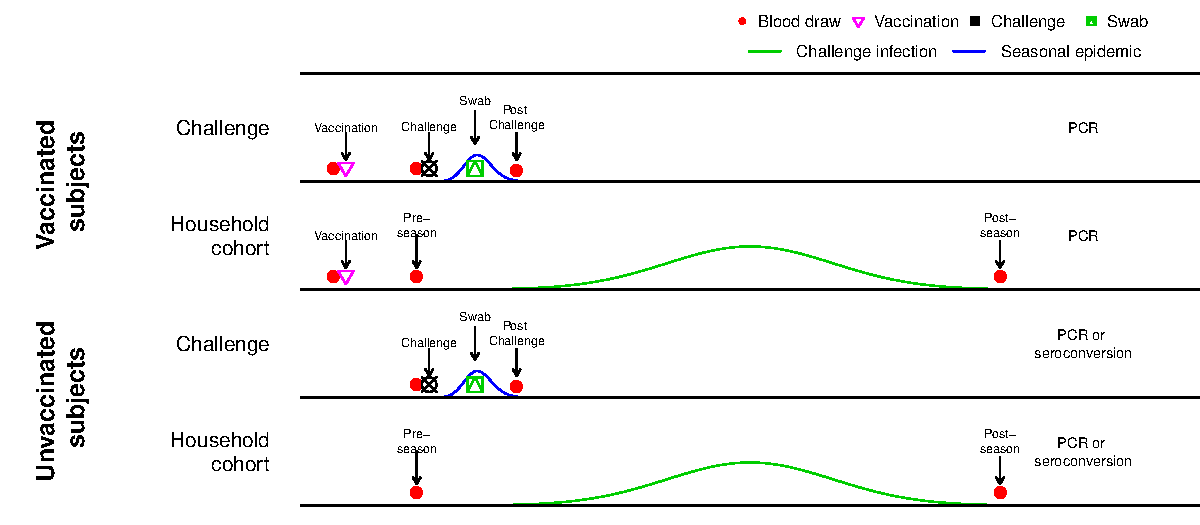
\includegraphics[width=\linewidth]{../fig-studies/fig-studies.pdf}
	\caption{\footnotesize
	Example study designs for the estimation of protective titres.
}
\label{Studies}
\end{figure}

\pagebreak
%==============================================================================
\section{Cox proportional hazards}

In Cox proportional hazards regression, the outcome considered is time to event. This time should normally be time at risk of an observable event. As an illustration, in Figure \ref{CoxExampleFull}, two subjects are followed until both experience an event (e.g. infection).

\begin{figure}[htp]
	\centering
	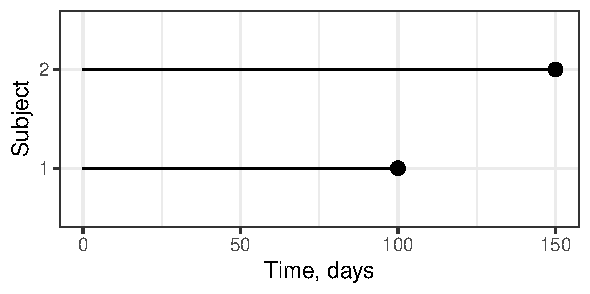
\includegraphics[width=0.6\textwidth]{../curve-cox/timeplot_1_light.pdf}
	\caption{
	An example of time to event data. Two subjects are followed from time 0. Subject 1 experiences the even at time 100. Subject 2 experiences the event at time 150.
	}
	\label{CoxExampleFull}
\end{figure}

Since subject 2 experienced the event later (i.e. ``survived'' for longer), the covariate pattern (e.g. antibody titre) of subject 2 would be considered by the model to be more ``protective'' than that of subject 1.

If subjects are not at risk of the event for all of their follow-up time (e.g. not exposed to the virus), then the total follow-up time may be misleading as illustrated in Figure \ref{CoxExamplePartial}. Taking the actual time at risk into account would lead to the opposite conclusion in this example --- it is subject 1 who is more ``protected'' since they were at risk for longer.

\begin{figure}[htp]
	\centering
	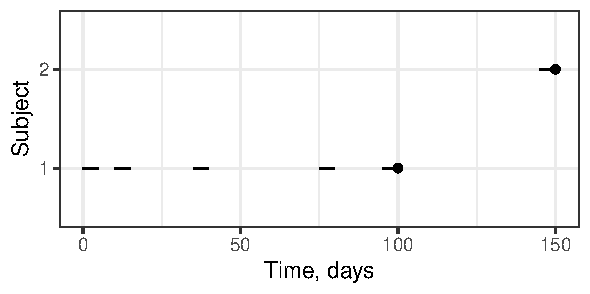
\includegraphics[width=0.6\textwidth]{../curve-cox/timeplot_2_light.pdf}
	\caption{
	An example of time to event data. Two subjects are followed from time 0. Subject 1 experiences the even at time 100. Subject 2 experiences the event at time 150. Subject 1 was at risk of the event for a total of 5 days. Subject 2 was at risk of the event for a total of 25 days.
	}
	\label{CoxExamplePartial}
\end{figure}

\pagebreak

In infection data, true time at risk is unobservable because the risk of infection among susceptible individuals depends on exposure to the pathogen, which cannot be controlled. If follow-up time is completely unrepresentative of true time at risk, the Cox model will not produce reliable results. However, if the total time of follow-up is assumed to be, on average, proportional to the total time at risk (e.g. subjects who are followed up for longer can be expected to have been exposed for longer) then the situation illustrated in Figure  \ref{CoxExamplePartial} will be ``averaged out'' and the model may still produce reliable results.

To investigate this, we generated a simulated dataset, based on the following model:

\begin{align*}
\begin{gathered}
T \sim \text{Exponential}(\text{rate} = \lambda) \\
h(t) = \lambda \\
\text{log}\lambda = -3 - 1.5 X_{\text{logtitre}}
\end{gathered}
\end{align*}

Where $T$ is the survival time, $h$ is the hazard and $X_{\text{logtitre}}$ is the true logtitre measurement simulated from $N(2, 2^2)$.

Each individual was assigned a proportion of time they were exposed to the virus. This proportion was generated from $\text{Beta}(10, 10\frac{1-m}{m})$ where $m$ is the expected proportion for the population. When $m$ was 1, the proportion assigned was always 1 to represent the ideal context of all follow-up time being time at risk. The maximum time of follow-up was set to 200 (days). If an individual's true survival time (a random number generated by $\text{Exponential}(\text{rate} = \text{exp}(-3 - 1.5 X_{\text{logtitre}}) )$ was at most 200 times their ``time at risk proportion'', then they were ``infected''. Otherwise, they were ``not infected''. 

Recorded time for each individual was 200 for everyone not infected (i.e. they were followed for the entire follow-up period and did not experience the event) and the true survival time divided by ``time at risk proportion'' for everyone infected (i.e. they were followed for that amount of time before experiencing the event).

Each simulation included 10,000 observations and was run 10,000 times at different values of the expected proportion of time at risk. The Cox proportional hazards model was fit to each simulated dataset. From 10,000 simulations at each value of the expected proportion at risk, the mean of the estimated coefficient (a measure of its expected value at that proportion) and its standard deviation (a measure of its expected standard error at that proportion and sample size) were saved. The results are summarised in Figure \ref{CoxSimResults}.

In the ideal case (proportion of time at risk set to 1) the estimate is unbiased and has the smallest error. As the proportion of time at risk decreases, bias is introduced while the error remains almost constant. When the proportion is small (less than 20\%), bias appears to decrease while error increases.

The maximum bias was less than 4\% away from the true value. The standard error increases notably only when the expected proportion at risk is very small (less than 10\%). This shows that under the assumption that the time of follow-up is proportional to time at risk, the Cox model can be expected to produce reliable results.

\begin{figure}[htp]
	\centering
	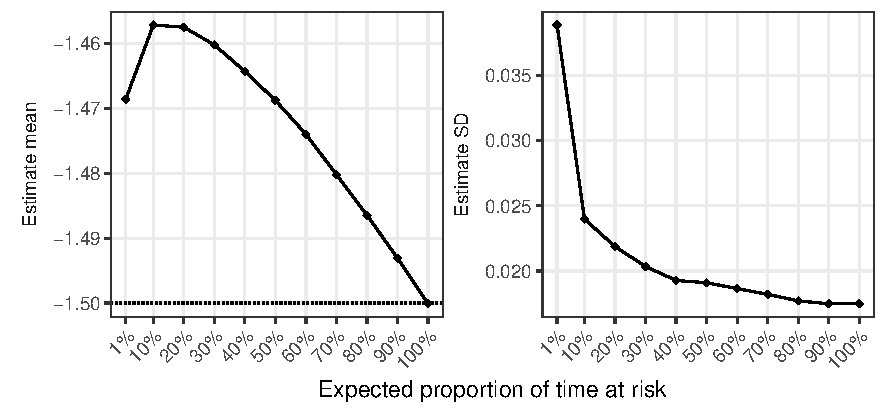
\includegraphics[width=1\textwidth]{../cox-tarprop-plot/risk.pdf}
	\caption{
	The results of time to event simulations. For each proportion of time at risk the mean of the estimated coefficient (left panel) is shown as well its standard deviation (right panel) obtained from 10,000 simulations. Points represent the values of expected proportion for which the simulations were performed. The dotted horizontal line is the true value of the estimated parameter.
	}
	\label{CoxSimResults}
\end{figure}

The assumption of time at risk being proportional to time of follow-up is likely to hold when everyone in the sample is followed through a period of similar disease activity. There may still be subjects who are not exposed (or over-exposed) but as long as the level of exposure does not correlate with the covariates of interest (e.g. antibody titres), then with a large enough sample size the average exposure for any covariate pattern (e.g. antibody titre level) should be proportional in the same way to the time of follow-up. If the disease is seasonal, the start of follow-up can be set to the start of the season. For those who do not get infected, end of follow-up can then be the end of the season. For those who do get infected, end of follow-up can be the infection time assuming that infection grants immunity for the rest of the season. An illustration is in Figure \ref{CoxIdeal}.

\begin{figure}[htp]
	\centering
	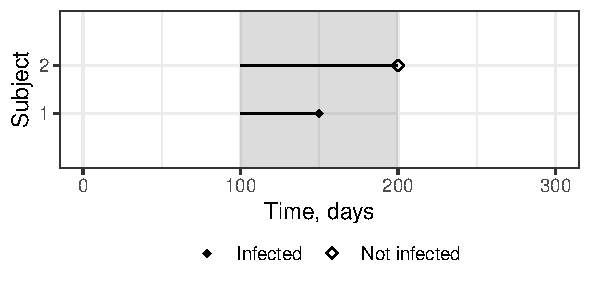
\includegraphics[width=0.59\textwidth]{../curve-cox/timeplot_3_light.pdf}
	\caption{
	An illustration of a pattern of follow-up where the assumption of true time at risk being proportional to time of follow-up is likely to hold. The shaded region marks the period of time when the disease is active. Both subject's follow-up starts at the beginning of the disease season (activity). Subject 1 gets infected at 150 days, their follow-up would end there assuming infection grants immunity (their total recorded time of follow-up would be 50 days). Subject 2 does not get infected through the season, their time of follow-up ends at the end of the season (their total recorded time of follow-up would be 100 days).
	}
	\label{CoxIdeal}
\end{figure}

The assumption will likely not hold if, with a seasonal disease, there are people in the sample whose follow-up starts before the season. An illustration is in Figure \ref{CoxNotIdeal}. For those with earlier follow-up start, their follow-up time will be large regardless of their titres (since they spend a proportion of that time not being at risk). This should make it seem like the titres have a smaller effect than they actually do thus biasing the estimate of titre effect towards the null.

\begin{figure}[htp]
	\centering
	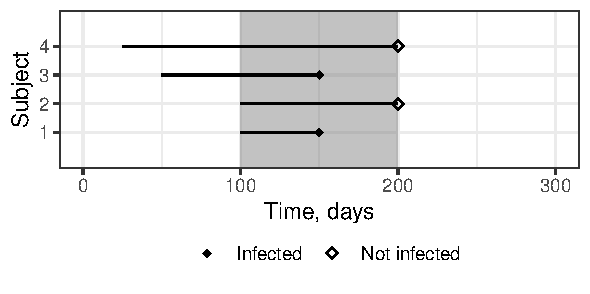
\includegraphics[width=0.59\textwidth]{../curve-cox/timeplot_4_light.pdf}
	\caption{
	An illustration of a pattern of follow-up where the assumption of true time at risk being proportional to time of follow-up is likely to not hold. The shaded region marks the period of time when the disease is active. Subject 1 gets infected at 150 days, at which point their follow-up would end if it can be assumed that infection grants immunity (their total recorded time of follow-up would be 50 days). Subject 2 does not get infected within the season, their follow-up ends at the end of the season (their total recorded time of follow-up would be 100 days). For subjects 3 (recorded follow up of 100 days) and 4 (recorded follow-up of 175 days) follow-up commenced prior to season onset.
	}
	\label{CoxNotIdeal}
\end{figure}

%\pagebreak

To demonstrate this problem, we performed some additional simulations using the same procedure as described above except subjects were randomly chosen to have had their follow-up started earlier. For those chosen, a uniform random number between 0 and 200 (days) was added to their recorded follow-up time. The proportion of time at risk was set to 1. The bias resulting from varying the proportion of the sample with earlier follow-up is shown in Figure \ref{CoxSimLong}. The estimate is unbiased when follow-up starts at the start of the season. Bias towards the null increases rapidly even when only a small (10\%) proportion of the sample has started follow-up prior to the season. For this reason, it would be advisable to record follow-up time in such a way so that true unobservable time at risk can be reasonably expected to be proportional to the recorded time of follow-up (i.e. the longer a subject is followed, the longer they are likely to have been at risk).

\begin{figure}[htp]
	\centering
	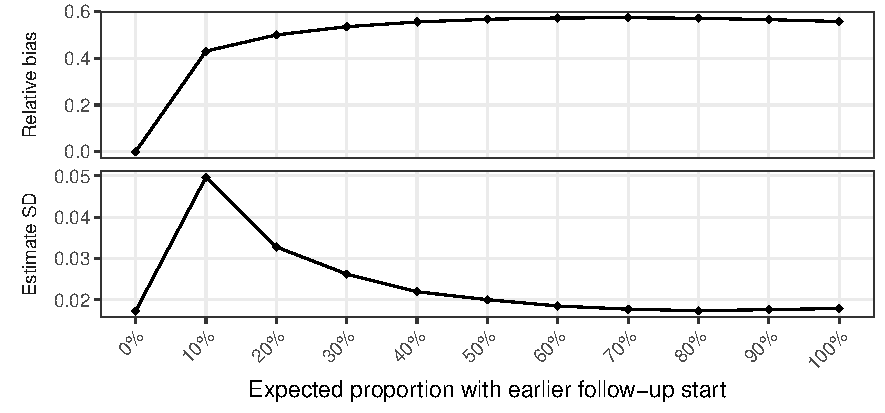
\includegraphics[width=1\textwidth]{../cox-tarprop-plot/long.pdf}
	\caption{
	The results of time to event simulations. For each proportion of the sample with earlier follow-up start, the mean of the estimated coefficient (left panel) is shown as well as the standard deviation of that coefficient (right panel) from 10,000 simulations. Points represent the values of expected proportion for which the simulations were performed. The dotted horizontal line is the true value of the estimated parameter.
	}
	\label{CoxSimLong}
\end{figure}

%\pagebreak
%==============================================================================
\section{Logistic regression}

The logistic model assumes that the probability of outcome follows a logistic curve from 1 (at low covariate values assuming a protective covariate) to 0 (at high covariate values). If there is only one covariate which is the antibody titre measurement, then the model is:

\begin{align*}
\begin{gathered}
P(Y=1) = \frac{\text{exp}(\beta_0 + \beta_T X_{\text{logtitre}})}{1 + \text{exp}(\beta_0 + \beta_T X_{\text{logtitre}})}
\end{gathered}
\end{align*}

A potentially large problem with the application of this model to antibody data is that low antibody titres do not necessarily guarantee infection (which is one of the model's assumptions). This assumption of baseline risk of 1 can be justified if it is shown that subjects with low antibody titres always (or almost always) get infected. If a large proportion of subjects with low titres do not get infected, this assumption is not justified. As an example, this assumption is not justified in the Ha Nam data as shown in Figure \ref{HanamCounts}. In both the general and the exposed populations, less than half the subjects with the titres below detectable levels (recorded as 5) were infected. %???during what time period?  I don't think we specified the period for which you have data

\begin{figure}[htp]
	\centering
	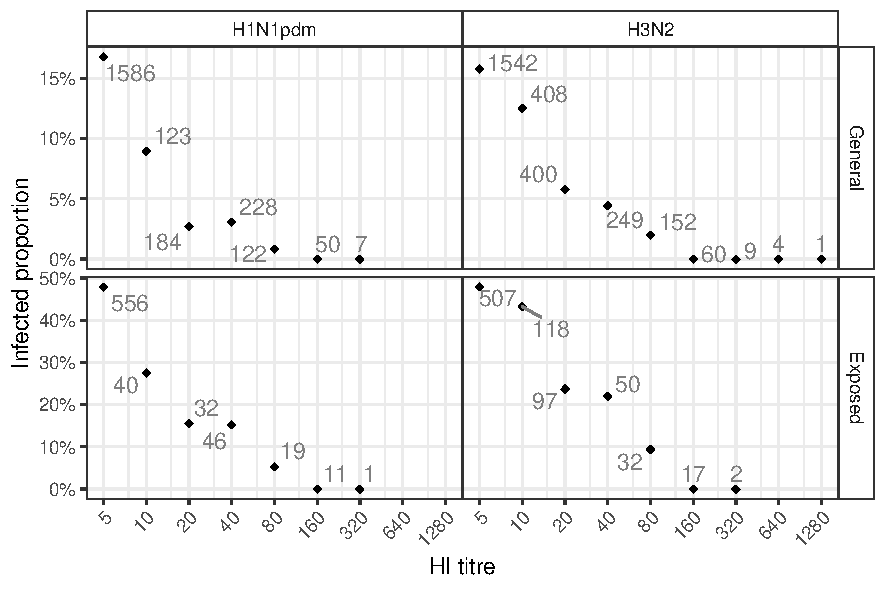
\includegraphics[width=0.9\textwidth]{../data-plot/hanam-hi-summ-light.pdf}
	\caption{
	Ha Nam cohort data. Subjects were grouped by virus and measured HI titre. Numbers next to points are the total number of observations in the corresponding group. The top row is all observations. The bottom row are the observations from households with at least one infection in a given season. The left column is observations for the H1N1pdm virus, the right row --- for H3N2 virus.
	}
	\label{HanamCounts}
\end{figure}

If baseline risk cannot justifiably be assumed to be 1, the fitted probability curve will be flatter than the true curve, thereby misrepresenting the true probability of infection across the titre range. An illustration is in Figure \ref{LogisticFit}. Thus, ignoring the baseline risk assumption will lead to biased estimates.


%\pagebreak

\begin{figure}[htp]
	\centering
	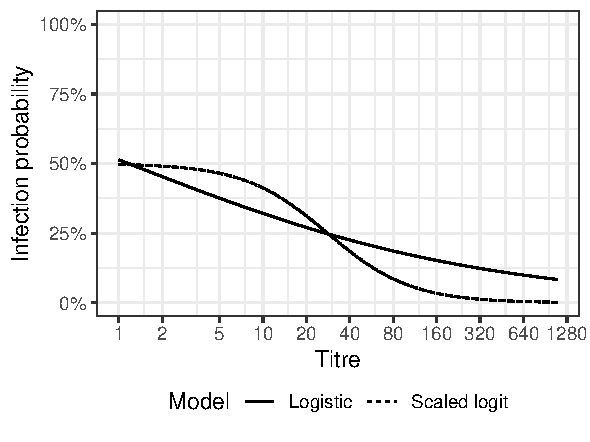
\includegraphics[width=0.6\textwidth]{../logistic-plot/lrex.pdf}
	\caption{
	An illustration of a bad fit of the logistic model. The dotted line (overlaps the dashed line) is the true probability curve $0.5\frac{\text{exp}(5 - 1.5 X_{\text{logtitre}})}{1 + \text{exp}(5 - 1.5 X_{\text{logtitre}})}$. The solid line is the expected fitted probability curve from standard logistic regression. The dashed line (overlaps the dotted line) is the expected fitted probability curve from scaled logistic regression. The expected curves was obtained from 10,000 simulations each with 10,000 observations simulated from the true curve. The models were fitted to each simulated dataset and the means of the regression estimates were taken from all simulations.
	}
	\label{LogisticFit}
\end{figure}


%\pagebreak
%==============================================================================
\section{Scaled logistic regression}

This model is the same as logistic regression except that it estimates the baseline probability of outcome (i.e. the probability at low covariate values assuming a protective covariate) as opposed to assuming that it is equal to 1. If there is only one covariate which is the antibody titre measurement then the model is

\begin{align*}
\begin{gathered}
P(Y=1) = \frac{\lambda}{1 + \text{exp}(\beta_0 + \beta_T X_{\text{logtitre}})}
\end{gathered}
\end{align*}

Note that with the above parameterisation, the $\beta$ parameters are negated relative to logistic regression.

The model still assumes that low probability bound is 0 (i.e. that high titres guarantee immunity in a univariate model). This assumption is justified if there is a reasonable number of people in the sample who have high titres and none (or very few) of whom get infected. In the Ha Nam data (Figure \ref{HanamCounts}), there is a total of 131 observations with titres above 160. None of those subjects got infected in the corresponding season justifying the assumption that high titres guarantee immunity.

Compared to logistic regression, the scaled logit model requires a larger sample size. This is because the scaled logit model attempts to use the same amount of information to estimate one more parameter. This leads to larger standard errors and potential convergence problems. Figures \ref{SclrSE} and \ref{SclrConv} summarise 10,000 simulation results from the model $\frac{0.5}{\text{exp}(-5 + 1.5 X_{\text{logtitre}})}$ with $X_{\text{logtitre}}$ simulated from $N(2, 2^2)$. Logistic and scaled logit models were fit using maximum likelihood estimation. 

Standard errors of the $\beta$ regression estimates ($\beta_0$ being the intercept and $\beta_T$ being $X_{\text{logtitre}}$ coefficient) were consistently higher with the scaled logit model. In order to reliably converge (under the chosen true parameter values) the scaled logit model required the sample size to be over 500. The standard logistic model always converged.

%\pagebreak

\begin{figure}[htp]
	\centering
	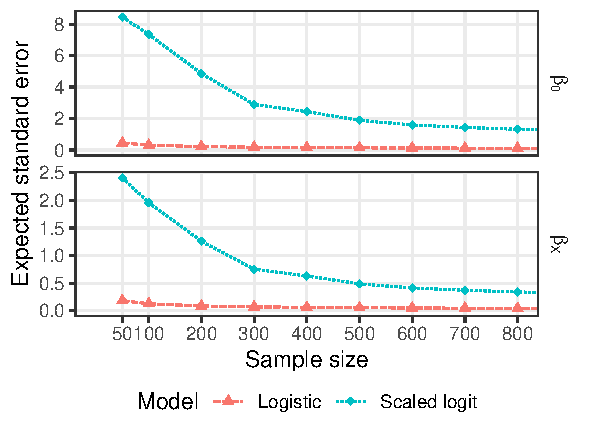
\includegraphics[width=0.69\textwidth]{../logistic-plot/vary_nsam_se.pdf}
	\caption{
	Simulation results of fitting the standard logistic and the scaled logit models to the same simulated datasets. 10,000 datasets were simulated. Shown is the mean standard deviation (estimate of the expected standard error) of the $\beta$ regression estimates from the standard logistic (the solid line) and the scaled logit (the dashed line). Points indicate parameter values at which the simulations were performed.
	}
	\label{SclrSE}
\end{figure}

\begin{figure}[H]
	\centering
	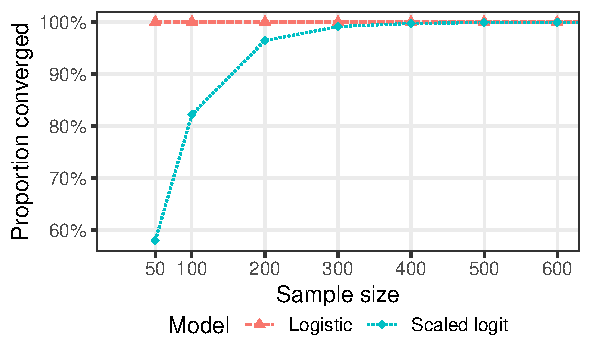
\includegraphics[width=0.69\textwidth]{../logistic-plot/vary_nsam.pdf}
	\caption{
	Simulation results of fitting the standard logistic and the scaled logit models to the same simulated datasets. 10,000 datasets were simulated. Shown is the proportion of successful attempts to fit the standard logistic (the solid line) and the scaled logit (the dashed line) model. Points indicate parameter values at which the simulations were performed.
	}
	\label{SclrConv}
\end{figure}

%\pagebreak
%==============================================================================
\section{Ha Nam application}

This section shows an application of the scaled logit model to the Ha Nam cohort which is plotted in Figure \ref{HanamCounts}. For this cohort, the Cox model is inapplicable due to absence of reliable data on disease activity. The standard logistic model is inappropriate due to unjustified assumption of baseline of 1.

%------------------------------------------------------------------------------
\subsection{Scaled logit fit}

The scaled logit model was fit using the maximum likelihood method. The fitted protection curves are in Figure \ref{fig:fit-sclr-prot}.

\begin{figure}[htp]
	\centering
	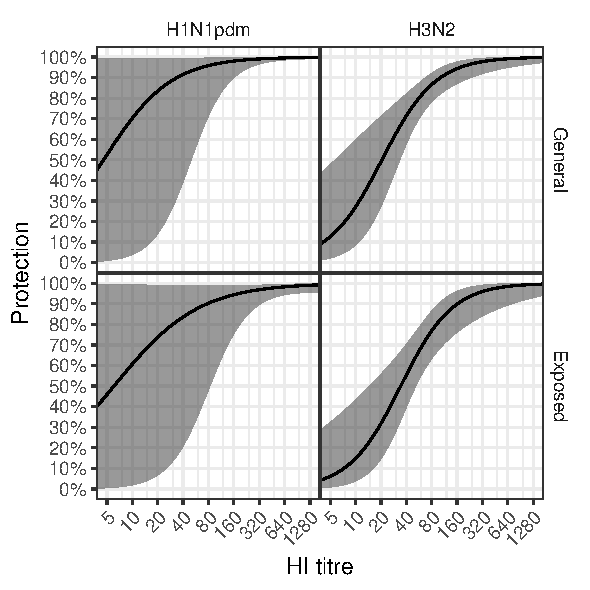
\includegraphics[width=0.8\textwidth]{../fit-sclr-plot/hanam-hi-prot.pdf}
	\caption{
	Fitted protection curves and confidence intervals from the scaled logit fit to Ha Nam data (also shown in Figure \ref{HanamCounts}) using the maximum likelihood method. The solid line is the point estimate. The shaded region is the 95\% confidence interval.
	}
	\label{fig:fit-sclr-prot}
\end{figure}

There is not enough data in the H1N1pdm subset to generate useful estimates. For H3N2 subset, limiting the sample to just those exposed to the virus (at least one household infection in a season) improved the precision of the estimates. The general lack of precision in the estimates is likely due to the number of parameters in the model (3 parameters with 1 covariate) and the censored nature of HI titre measurements, particularly the fact that any titre below 10 is undetectable which means that it is impossible to distinguish between many of the observations (e.g. some subjects with undetectable titres may have had a true titre of 9 while others --- of 2, but both were recorded as 5) which makes it harder to estimate the baseline probability (as seen in the confidence bounds increasing at small (<10) titres).

%\pagebreak
%------------------------------------------------------------------------------
\subsection{Comparison to standard logistic fit}

As mentioned before, the standard logistic model is inappropriate due to unsatisfied assumption of baseline of 1. It was fit to the same Ha Nam data using maximum likelihood with no accounting for censored titres (observations of 5 (below detectable) and 1280 (above detectable) were unchanged, all other observations were moved to the midpoint of the corresponding censored interval on a log scale). The fitted infection curve is in Figure \ref{lr-inf}.
-ba
\begin{figure}[htp]
	\centering
	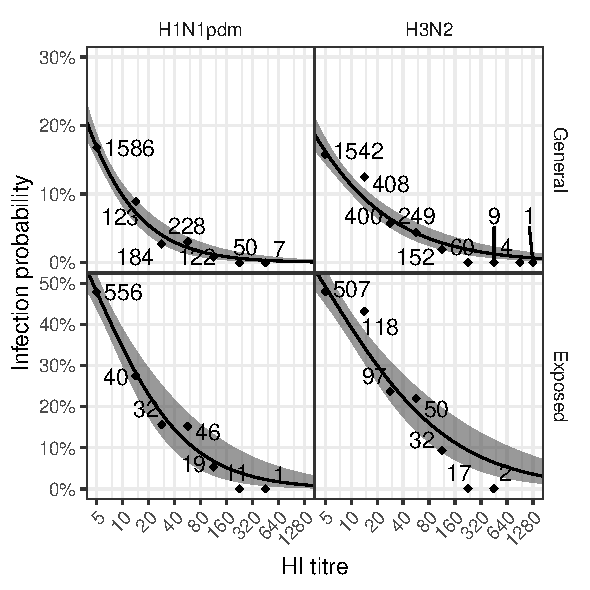
\includegraphics[width=0.8\textwidth]{../fit-logistic-plot/hanam-hi-inf.pdf}
	\caption{
	Fitted infection curves and confidence intervals from the standard logistic model fit to Ha Nam data (also shown in Figure \ref{HanamCounts}) using maximum likelihood with no accounting of censored titres (observations of 5 (below detectable) and 1280 (above detectable) were unchanged, all other observations were moved to the midpoints of the corresponding censored intervals on a log scale). The points are the infected proportions at the corresponding modified titre measurements (i.e. interval midpoints). The solid line is the point estimates. The shaded region is the 95\% confidence interval. The numbers next to the points are the total sample size of the corresponding groups.
	}
	\label{lr-inf}
\end{figure}

\pagebreak

While the infection curves appear to fit the data well, it is problematic to generate a protection curve from these results. There are two options for the protection curve. One is to use the same procedure as was used in the scaled logit fit --- divide the fitted infection probabilities by the baseline (here assumed to be 1, so the fitted values would not change) and subtract the resulting relative-to-baseline infection probabilities from 1. The protection curves resulting from this procedure are in Figure \ref{lr-prot-abs}.

\begin{figure}[htp]
	\centering
	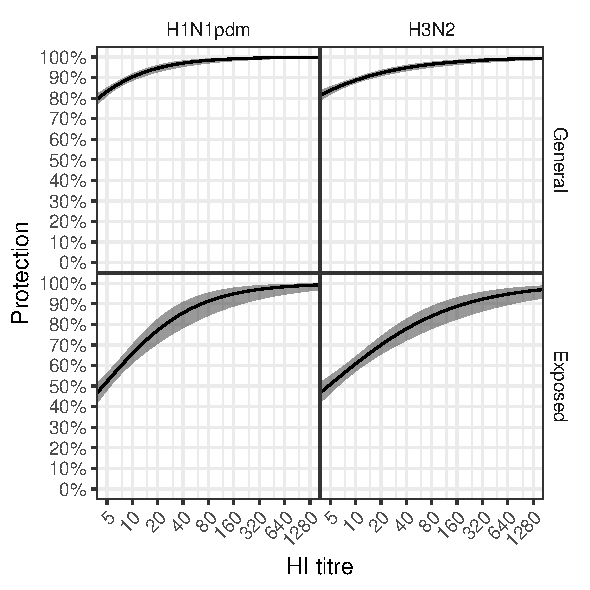
\includegraphics[width=0.8\textwidth]{../fit-logistic-plot/hanam-hi-prot.pdf}
	\caption{
	Fitted protection curves and confidence intervals from the standard logistic model fit to Ha Nam data (also shown in Figure \ref{HanamCounts}) using maximum likelihood with no accounting of censored titres (observations of 5 (below detectable) and 1280 (above detectable) were unchanged, all other observations were moved to the midpoints of the corresponding censored intervals on a log scale). The solid line is the point estimates. The shaded region is the 95\% confidence interval.
	}
	\label{lr-prot-abs}
\end{figure}

The other option for generating a protection curve is to calculate the fitted probability of infection at a give titre and divide that by the fitted probability of infection at the titre of 5 (or any other) thereby generating a curve that shows relative-to-5 infection probabilities (as opposed to relative-to-baseline). The variance of this quantity may be estimated by using the bootstrap method. Subtracting these relative-to-5 infection probabilities from 1 generates curves shown in Figure \ref{lr-prot-rel}.

\pagebreak

\begin{figure}[htp]
	\centering
	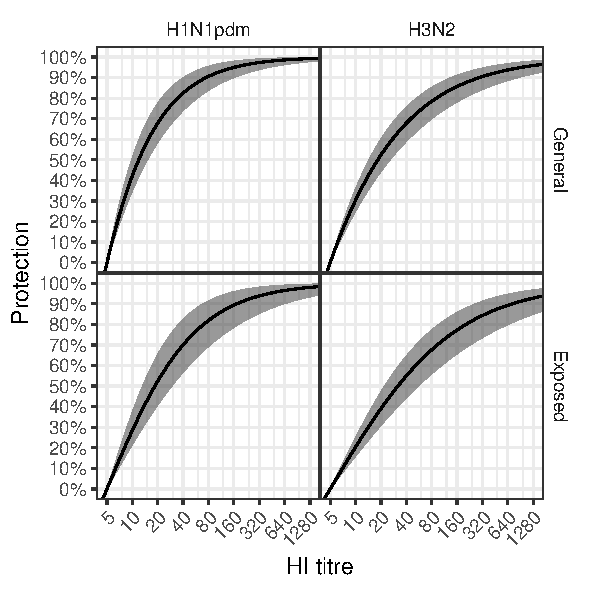
\includegraphics[width=0.8\textwidth]{../fit-logistic-boot-plot/hanam-hi-prot-rel.pdf}
	\caption{
	Fitted relative-to-5 protection curves and confidence intervals from the standard logistic model fit to Ha Nam data (also shown in Figure \ref{HanamCounts}) using maximum likelihood with no accounting of censored titres (observations of 5 (below detectable) and 1280 (above detectable) were unchanged, all other observations were moved to the midpoints of the corresponding censored intervals on a log scale). Solid lines are the point estimates, with shaded regions the 95\% confidence interval. The bounds for the confidence interval were obtained by using the bootstrap method (10,000 samples).
	}
	\label{lr-prot-rel}
\end{figure}

While the relative-to-5 protection curves (Figure \ref{lr-prot-rel}) appear more plausible than the relative-to-baseline protection curves (Figure \ref{lr-prot-abs}), both result from fitting a model with an unsatisfied assumption and neither method of generating protection curves from logistic regression model reliably produce accurate results.

The relative-to-5 curve (Figure \ref{lr-prot-rel}) presents an additional problem. The curve shows how much ``better'' different titres are at protecting against infection than the titre of 5. 
There is nothing inherently special about this threshold of 5. Its choice is based on the lower dilution of 10. Pre-treatment of the sera necessitates dilution, so the lower bound can never be 1, but could be something more than 1 such as <5.  Nevertheless, the curves may look substantially different if a different threshold (e.g. 10 or 1) is chosen.

\pagebreak
%==============================================================================
\section{Kiddyvax application}

The data for this study includes post-vaccination HI titres of subjects who were followed for up to one year for flu infection. The infection status was determined by PCR which was done for everyone who experienced symptoms. This data is shown in Figure \ref{fig:kiddyvax-main-titre}.

\begin{figure}[htp]
	\centering
	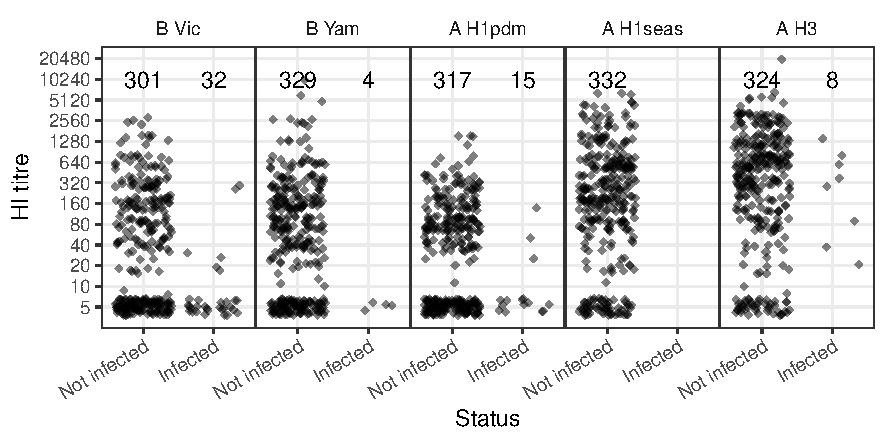
\includegraphics[width=1\textwidth]{../data-plot/kiddyvax-main-titre.pdf}
	\caption{
	Kiddyvax study data. Post-vaccination titres are shown for those who got infected (PCR-confirmed symptomatic infection) over the course of the study and those who did not. Panels correspond to the five tested viruses.
	}
	\label{fig:kiddyvax-main-titre}
\end{figure}

Analyses were done on the data for B Vic and A(H1pdm) viruses in the same way as for the Ha Nam data with the addition of the Cox proportional hazards model.

%\pagebreak
%
\subsection{Scaled logit fit}

The same scaled logit model was fit in the same way as for the Ha Nam data. The protection curves are in Figure \ref{fig:kiddyvaxmain-sclr-prot}. The model fails to produce useful estimates due to there being very few infections in the sample.

\begin{figure}[htp]
	\centering
	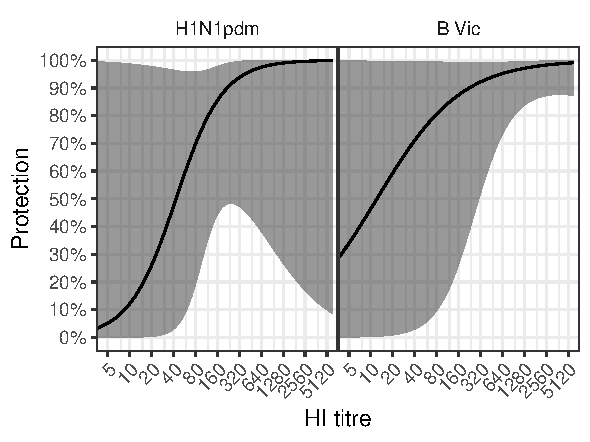
\includegraphics[width=0.8\textwidth]{../fit-sclr-plot/kiddyvaxmain-prot.pdf}
	\caption{
	Fitted protection curves and confidence intervals from the scaled logit fit to Kiddyvax data (also shown in Figure \ref{fig:kiddyvax-main-titre}) using the maximum likelihood method. The solid line is the point estimate. The shaded region is the 95\% confidence interval.
	}
	\label{fig:kiddyvaxmain-sclr-prot}
\end{figure}

%\pagebreak
%
\subsection{Standard logistic fit}

The relative protection curves are in Figure \ref{fig:kiddyvaxmain-prot-rel-lr-boot}. The same considerations regarding the unjustified assumption of baseline risk of 1 apply here as they did with Ha Nam (Figure \ref{fig:kiddyvax-main-titre} shows many uninfected subjects with undetectable titres).

\begin{figure}[htp]
	\centering
	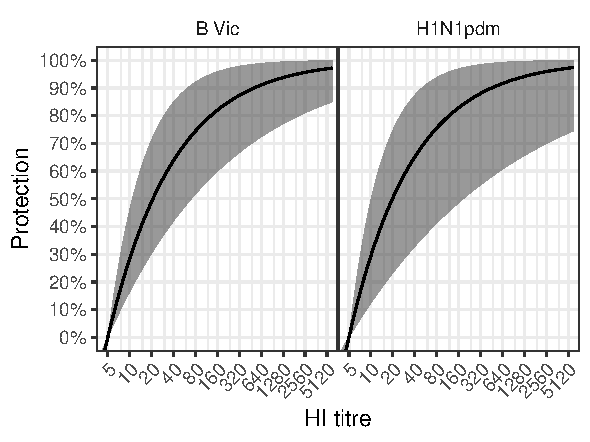
\includegraphics[width=0.8\textwidth]{../fit-logistic-boot-plot/kiddyvaxmain-prot-rel.pdf}
	\caption{
	Fitted relative-to-5 protection curves and confidence intervals from the standard logistic model fit to kiddyvax data (shown in Figure \ref{fig:kiddyvax-main-titre}) using maximum likelihood with no accounting of censored titres (observations of 5 (below detectable) were unchanged, all other observations were moved to the midpoints of the corresponding censored intervals on a log scale). The solid line is the point estimates. The shaded region is the 95\% confidence interval. The bounds for the confidence interval were obtained by using the bootstrap method (10,000 samples).
	}
	\label{fig:kiddyvaxmain-prot-rel-lr-boot}
\end{figure}

%\pagebreak
%------------------------------------------------------------------------------
\subsection{Cox proportional hazards fit}

For infected individuals, the time at risk was taken to be the time from start of follow-up to infection. For those who did not get infected the time at risk was take to be the time from start of follow-up to end of follow-up.

The model was

\begin{align*}
\begin{gathered}
h(t) = h_0\text{exp}(\beta_T X_{\text{logtitre}})
\end{gathered}
\end{align*}

where $h$ is the hazard function and $X_{\text{logtitre}}$ is the post-vaccination titre measurement on the log scale. The resulting protection curves (relative to the titre of 5) are in Figure \ref{fig:kiddyvaxmain-cox}. Although the point estimates are similar to those recovered from the model; however standard errors are inflated.

\begin{figure}[htp]
	\centering
	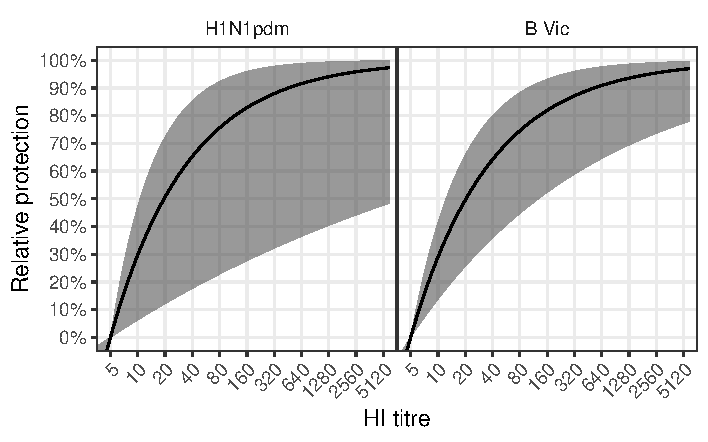
\includegraphics[width=0.8\textwidth]{../fit-cox-plot/kiddyvaxmain.pdf}
	\caption{
	Fitted relative-to-5 protection curves and confidence intervals from the Cox proportional hazards model fit to kiddyvax data (shown in Figure \ref{fig:kiddyvax-main-titre}) with no accounting of censored titres (observations of 5 (below detectable) were unchanged, all other observations were moved to the midpoints of the corresponding censored intervals on a log scale). The solid line is the point estimates. The shaded region is the 95\% confidence interval.
	}
	\label{fig:kiddyvaxmain-cox}
\end{figure}

\pagebreak
%
\section{Conclusion}

\begin{table}[htp]
\centering
\caption{Summary of the three considered models in terms of their application to antibody data}
\begin{tabular}{cp{25em}}
\toprule
Model & Potential problem \\
\midrule
Cox PH & Biased if follow-up time is not proportional to time at risk for everyone in the sample \\
Logistic & Biased if low antibody titres do not guarantee immunity \\
Scaled logit & Requires a large sample size. \\
\bottomrule
\end{tabular}
\end{table}

In this paper we have explored three different models for estimating protective antibody titres using data from influenza vaccine and infection studies.  We have shown that in the presence of good time-to-event data where every subject's follow-up time is at least proportional to their time at risk, the Cox model will likely perform best out the three models explored due to it having the least number of parameters allowing for more precise estimates. Absent such data, logistic regression may be appropriate if the assumption of everyone being infected at low antibody titres can be justified. If this assumption cannot be justified, which is probably the case for influenza studies, the scaled logit model can be applied but the sample needs to be fairly large (>500) in order to obtain useful estimates.

\pagebreak
\bibliography{bibliography}
All code is in github.com/khvorov45/model-comparison

\end{document}
